\FloatBarrier
\section{Time-of-Flight Detectors}\label{sec:clas.tof}

The \abbr{CLAS} time-of-flight \abbr{TOF} subsystem provides precise timing measurements of charged particles that transverse the \abbr{CLAS} detector to help determine the particle masses. The \abbr{TOF} subsystem was also used in the \g12 level 1 trigger (see Sec.~\ref{sec:data.trig}) to identify track candidates. The \abbr{TOF} is constructed of organic plastic scintillant (Bicron BC-408). Scintillation is a process undergone by material when radiation traverses a medium.
%
% At room temperature, all valence electrons of the scintillating material are in the $\mathrm{S_{0}}$ ground state. As a particle propagates through the material the incident radiation populates $\mathrm{S_{1}}$ states. Vibrational levels within $\mathrm{S_{1}}$ band decay radiation-less to $\mathrm{S_{1}}$  base states, which in turn decays under emission of light to the $\mathrm{S_{0}}$ band. The radiation-less decay from the excited $\mathrm{S_{1}}$ band to the ground $\mathrm{S_{1}}$ band is known as internal degradation and is responsible for the transparency of the scintillators to their own radiation. $\mathrm{S_{1}}$ can also decay to adjacent triplet levels however, this decay is highly forbidden by multipole selection rules. If this decay does occur, the decay energy is lower causing the decay time to be longer, see Fig.~\ref{fig:clas.scint_bands} for the illustration of this process. Depending on the properties of the scintillator, decay of fluorescent state in organic plastic scintillators have a typical time between 1-3~ns
%
%%\begin{figure}[h!]\begin{center}
%%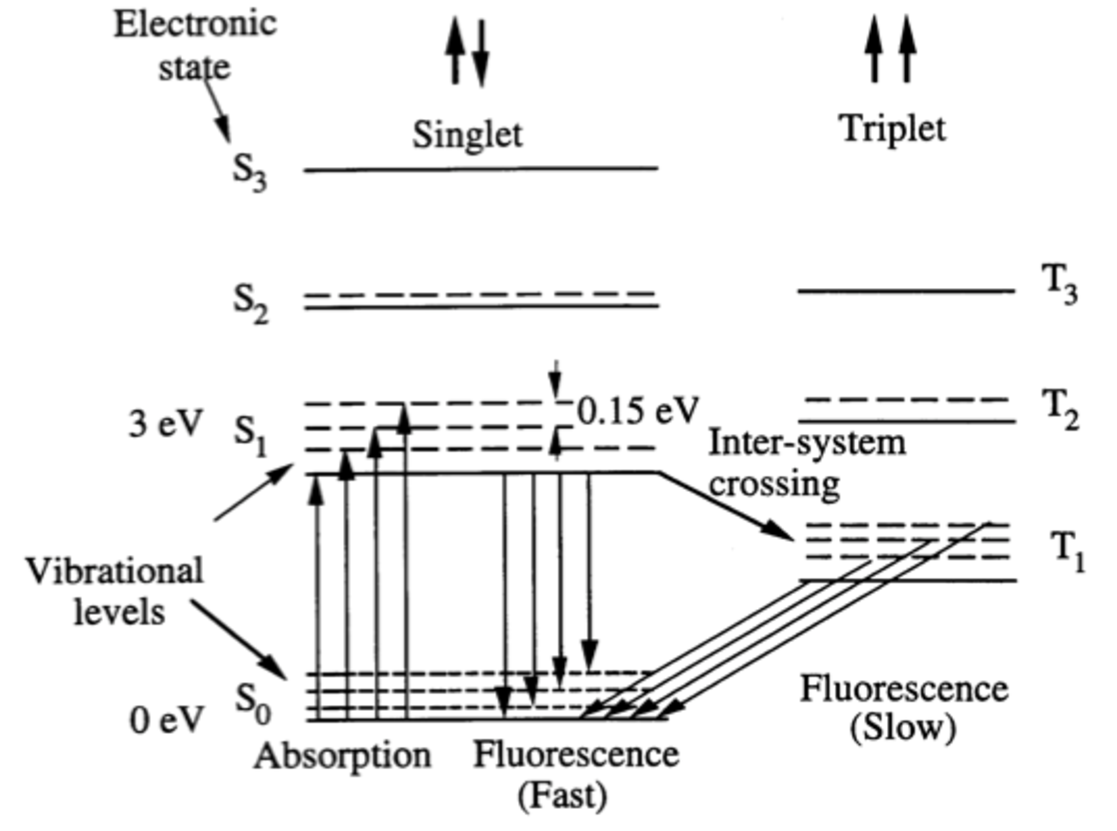
\includegraphics[width=\figwidth,height=0.5\hfigheight]{\figures/hall-b/CCECPLOTS/Calorimetry/scint.pdf}\label{fig:clas.scint_bands}\caption[Typical Energy Levels of scintillating material ]{Diagram of scintillating population of states. Image Source~\cite{vibe_levels}}
%%\end{center}\end{figure}
%\begin{figure}[h!]\begin{center}
%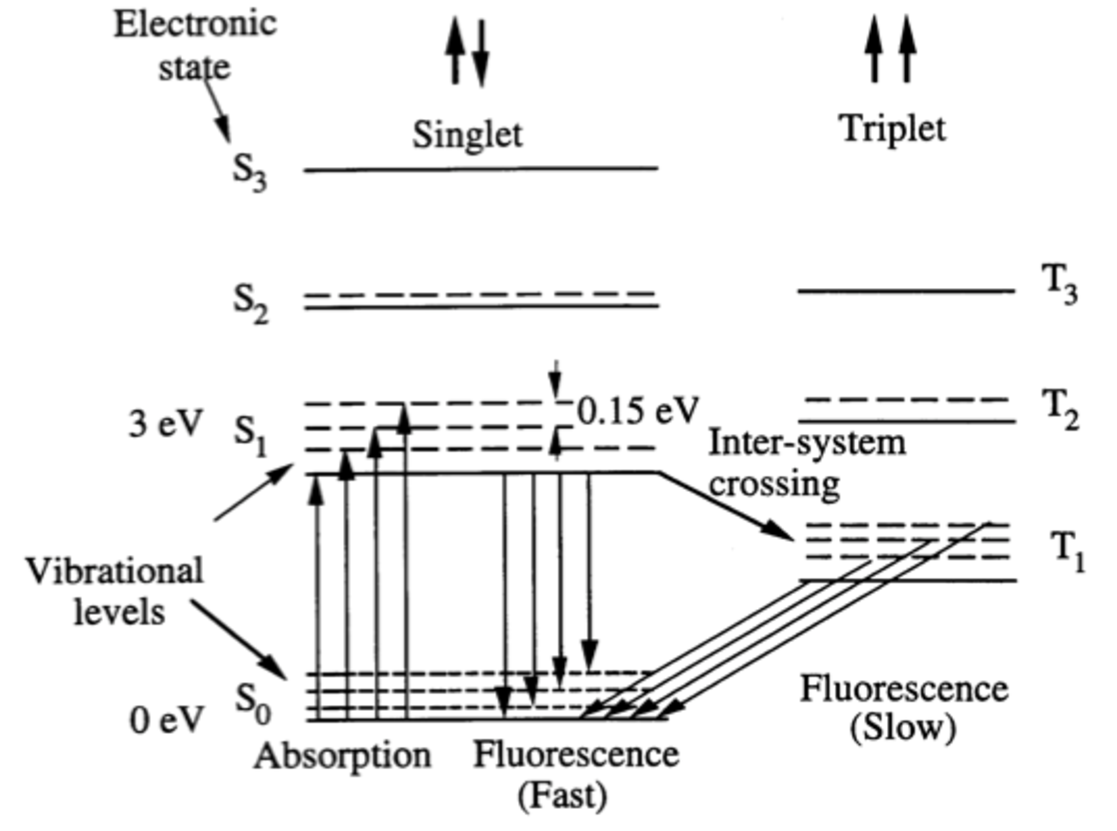
\includegraphics[width=\figwidth,height=0.5\hfigheight]{\figures/hall-b/CCECPLOTS/Calorimetry/scint.pdf}
%\caption[Typical Energy Levels of scintillating material ]{\label{fig:clas.scint_bands}Diagram of scintillating population of states. Image Source~\cite{vibe_levels}}
%\end{center}\end{figure}

The \abbr{TOF} subsystem is located between the \abbr{CC} and \abbr{EC} subsystems approximately 4~m from \abbr{CLAS} center, 5~m from the \g12 target. Each sector 57 scintillator paddles divided into two subgroups. The first subgroup subtends angles of 8.6$^\circ$ to 45.9$^\circ$ and consists of 23 scintillating paddles that are 15~cm in width. Each paddle is instrumented with two 2-in diameter \abbr{PMT}'s, see Fig~\ref{fig:clas.tof.paddles}. The first group was optimized for timing resolution while being cost-effective and covering a large area. The second group consists of 34 paddles that are 22~cm wide, covering polar angles from 45.9$^\circ$ to 142$^\circ$. Each paddle in this range is instrumented with two 3-in diameter \abbr{PMT}'s. All paddle bars are 5.08~cm thick for 100\% detection of minimum-ionizing tracks and a timing resolution of 150--200~ps.
%These forward angle counters \abbr{PMT}'s have a 15.9~cm$^2$ photocathode area which covers the 76.2~cm$^2$ cross-sectional area of the scintillator.
%These large angle counter \abbr{PMT}'s have a 30.2~cm$^2$ photocathode area which covers the 118.8~cm$^{\mathrm{2}}$ cross-sectional area of the scintillator.
\abbr{TOF} information is used to reconstruct a particle's mass is by measuring the difference between the event RF corrected start time and the time measured by the \abbr{TOF}, $t_{stsc}$. The RF corrected start time is the radio-frequency time (RF) from the accelerator beam aligned withe the event start time. Using this time, $t_{stsc}$, the length of trajectory to the \abbr{TOF}, $l_{stsc}$, and the speed of light $c$, the particles' velocity can be calculated as
\begin{equation}\label{eq:beta.cal}
\beta = l_{sc}/(t_{c}\cdot c)
\end{equation}
The particle's mass can be reconstructed from the measured velocity and momentum:
%Once the particles velocity is determined as well as the momentum, from the \abbr{DC} subsystem,  the particle mass can be reconstructed as 
\begin{equation}\label{eq:mass.cal}
m = p\sqrt{(1-\beta^2)}/\beta
\end{equation}

\begin{figure}\begin{center}
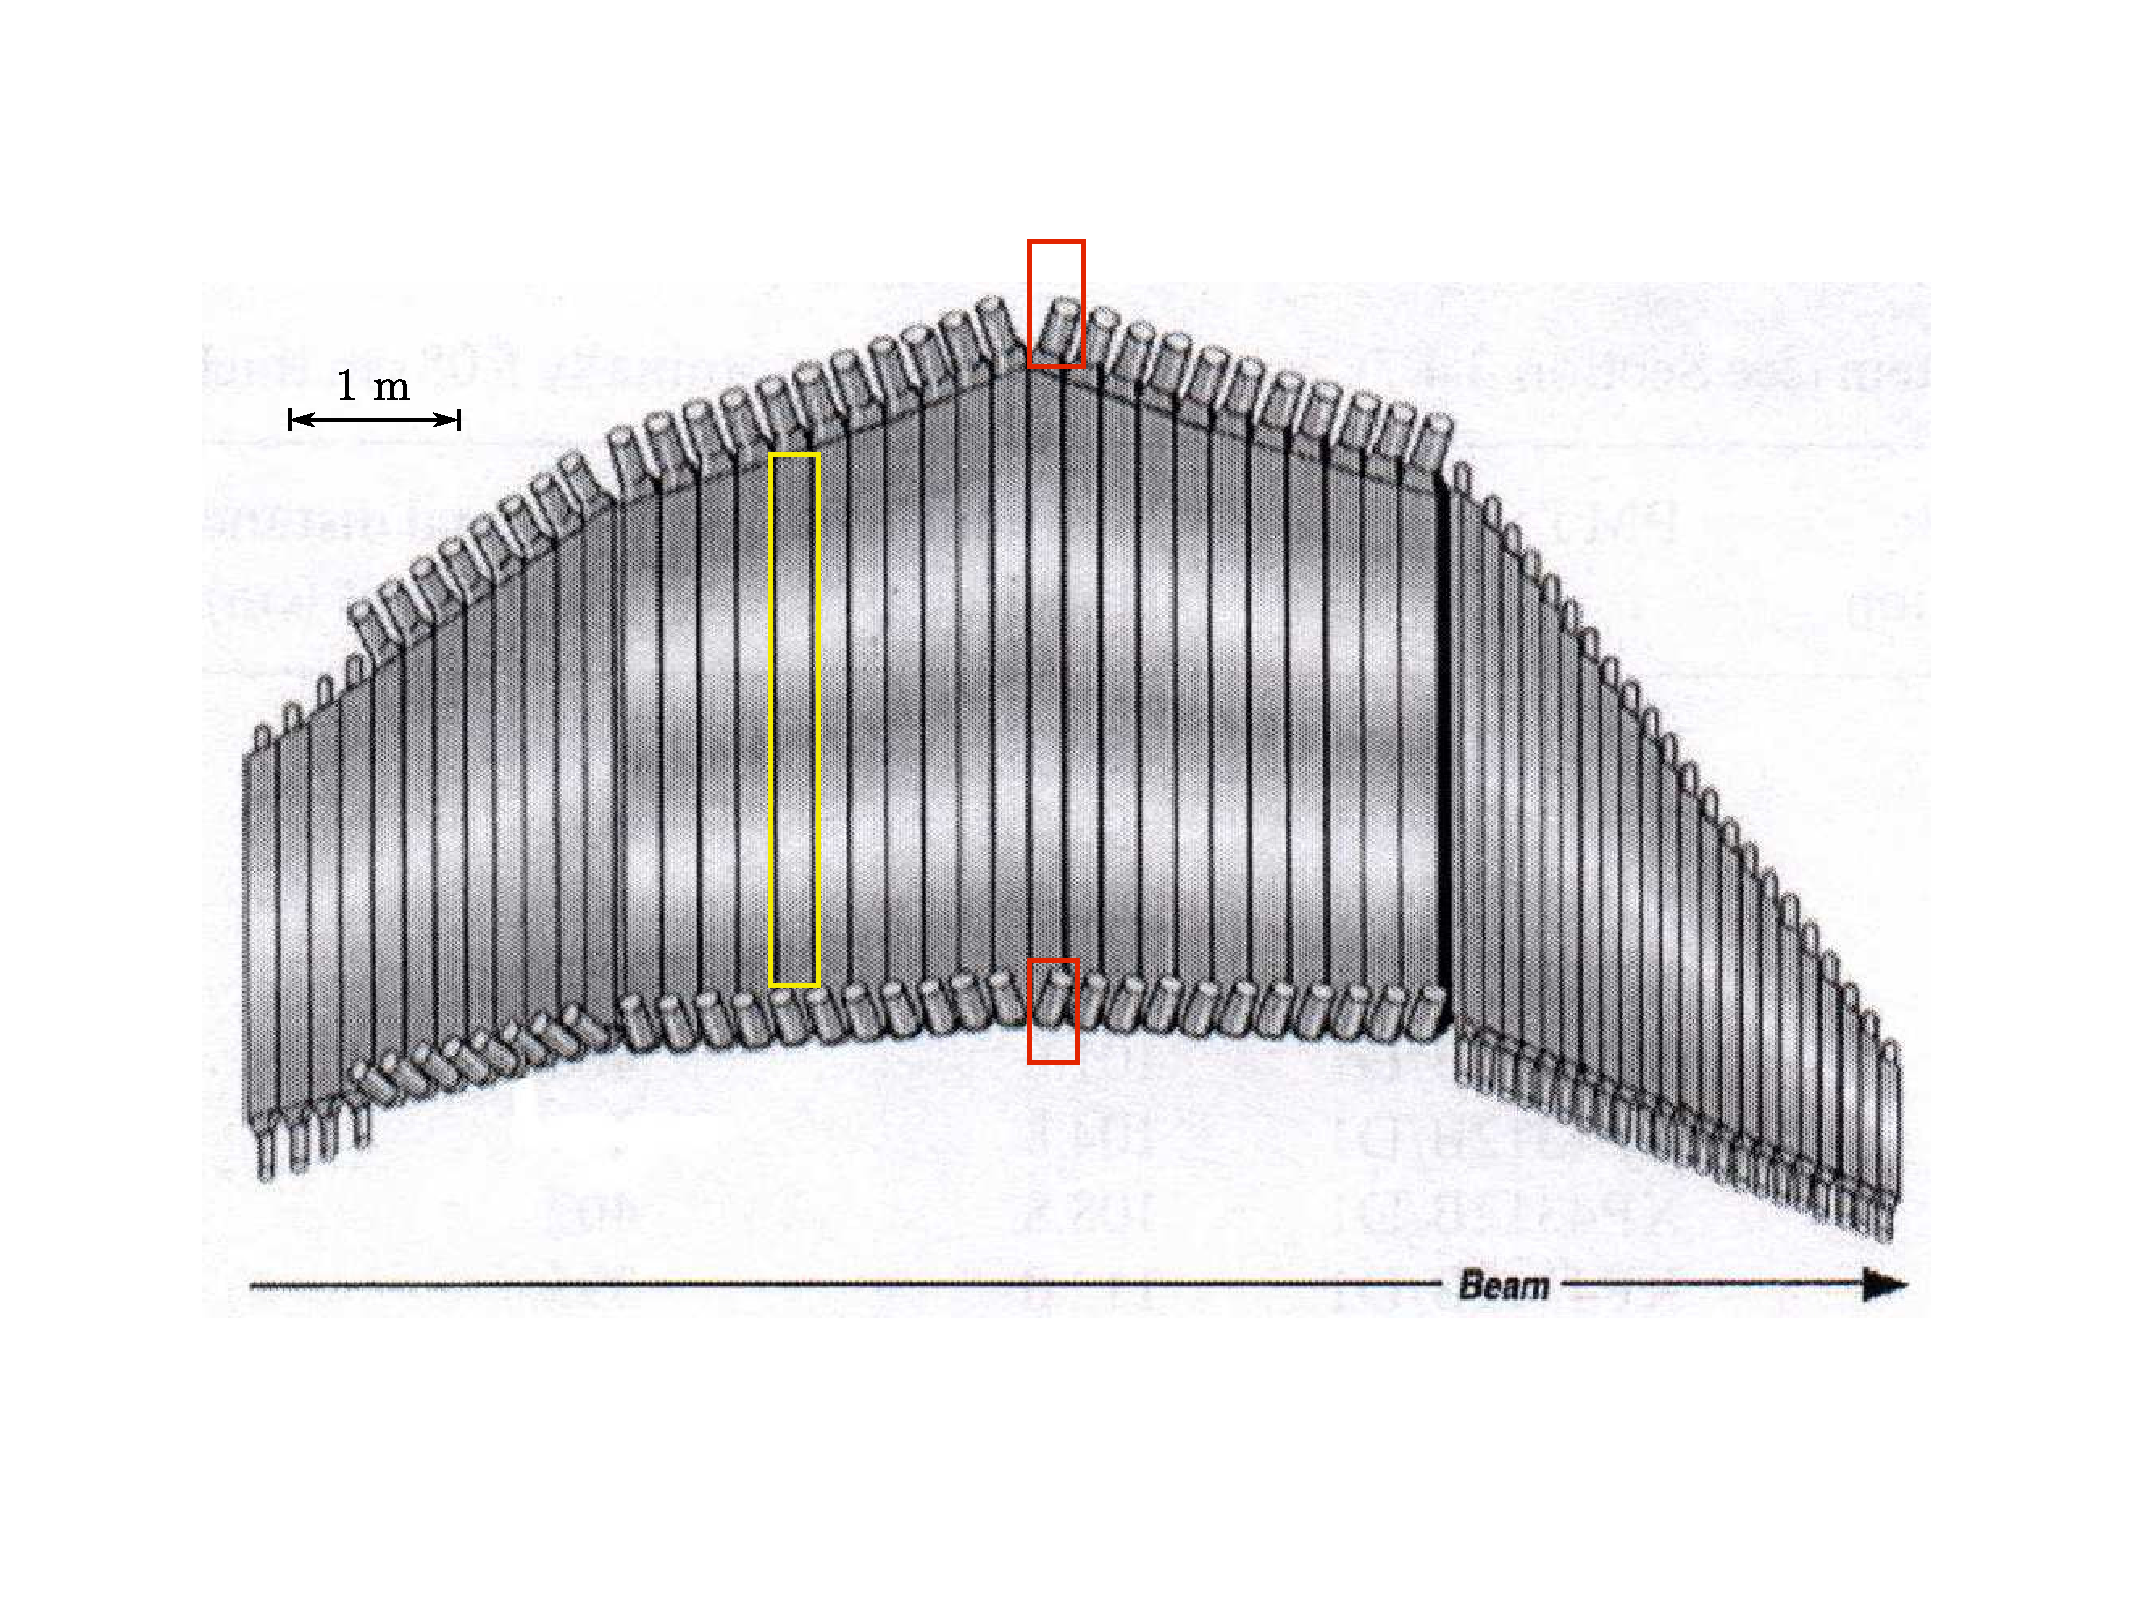
\includegraphics[width=\figwidth]{\figures/hall-b/tof_paddlesII.pdf}
\caption[Diagram of one sector of the time-of-flight (\abbr{TOF}) paddles]{\label{fig:clas.tof.paddles}Diagram of one sector of the time-of-flight (\abbr{TOF}) paddles. There are 57 scintillator paddles covering the entire acceptance region of the drift-chambers for each sector. \abbr{PMT}'s are outlined in red while a scintillator paddle is outlined in yellow.  Image Source:~\cite{clas.tof}}
\end{center}\end{figure}

\FloatBarrier
%\begin{figure}\begin{center}
%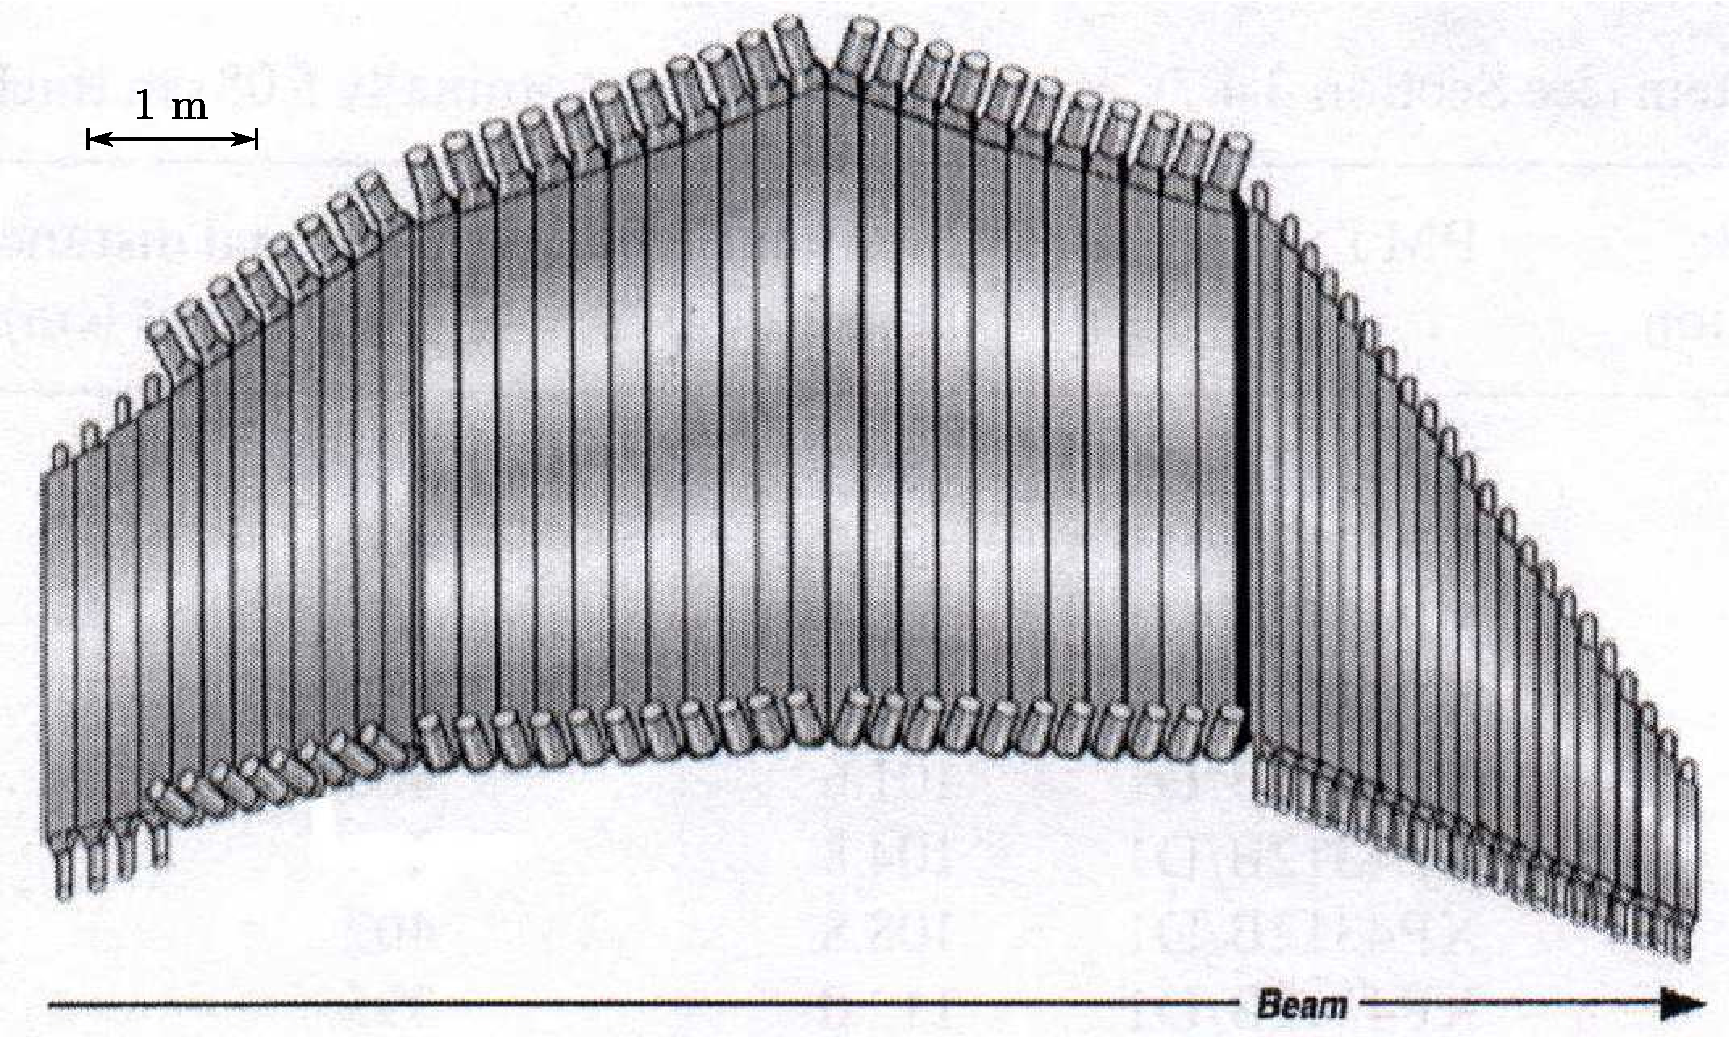
\includegraphics[width=\figwidth]{\figures/hall-b/tof_paddles.pdf}
%\caption[Time-of-Flight Paddles]{\label{fig:clas.tof.paddles}Diagram of one sector of the time-of-flight (\abbr{TOF}) paddles. There are 57 scintillator paddles covering the entire acceptance region of the drift-chambers for each sector.}
%\end{center}\end{figure}
%
%\begin{figure}\begin{center}
%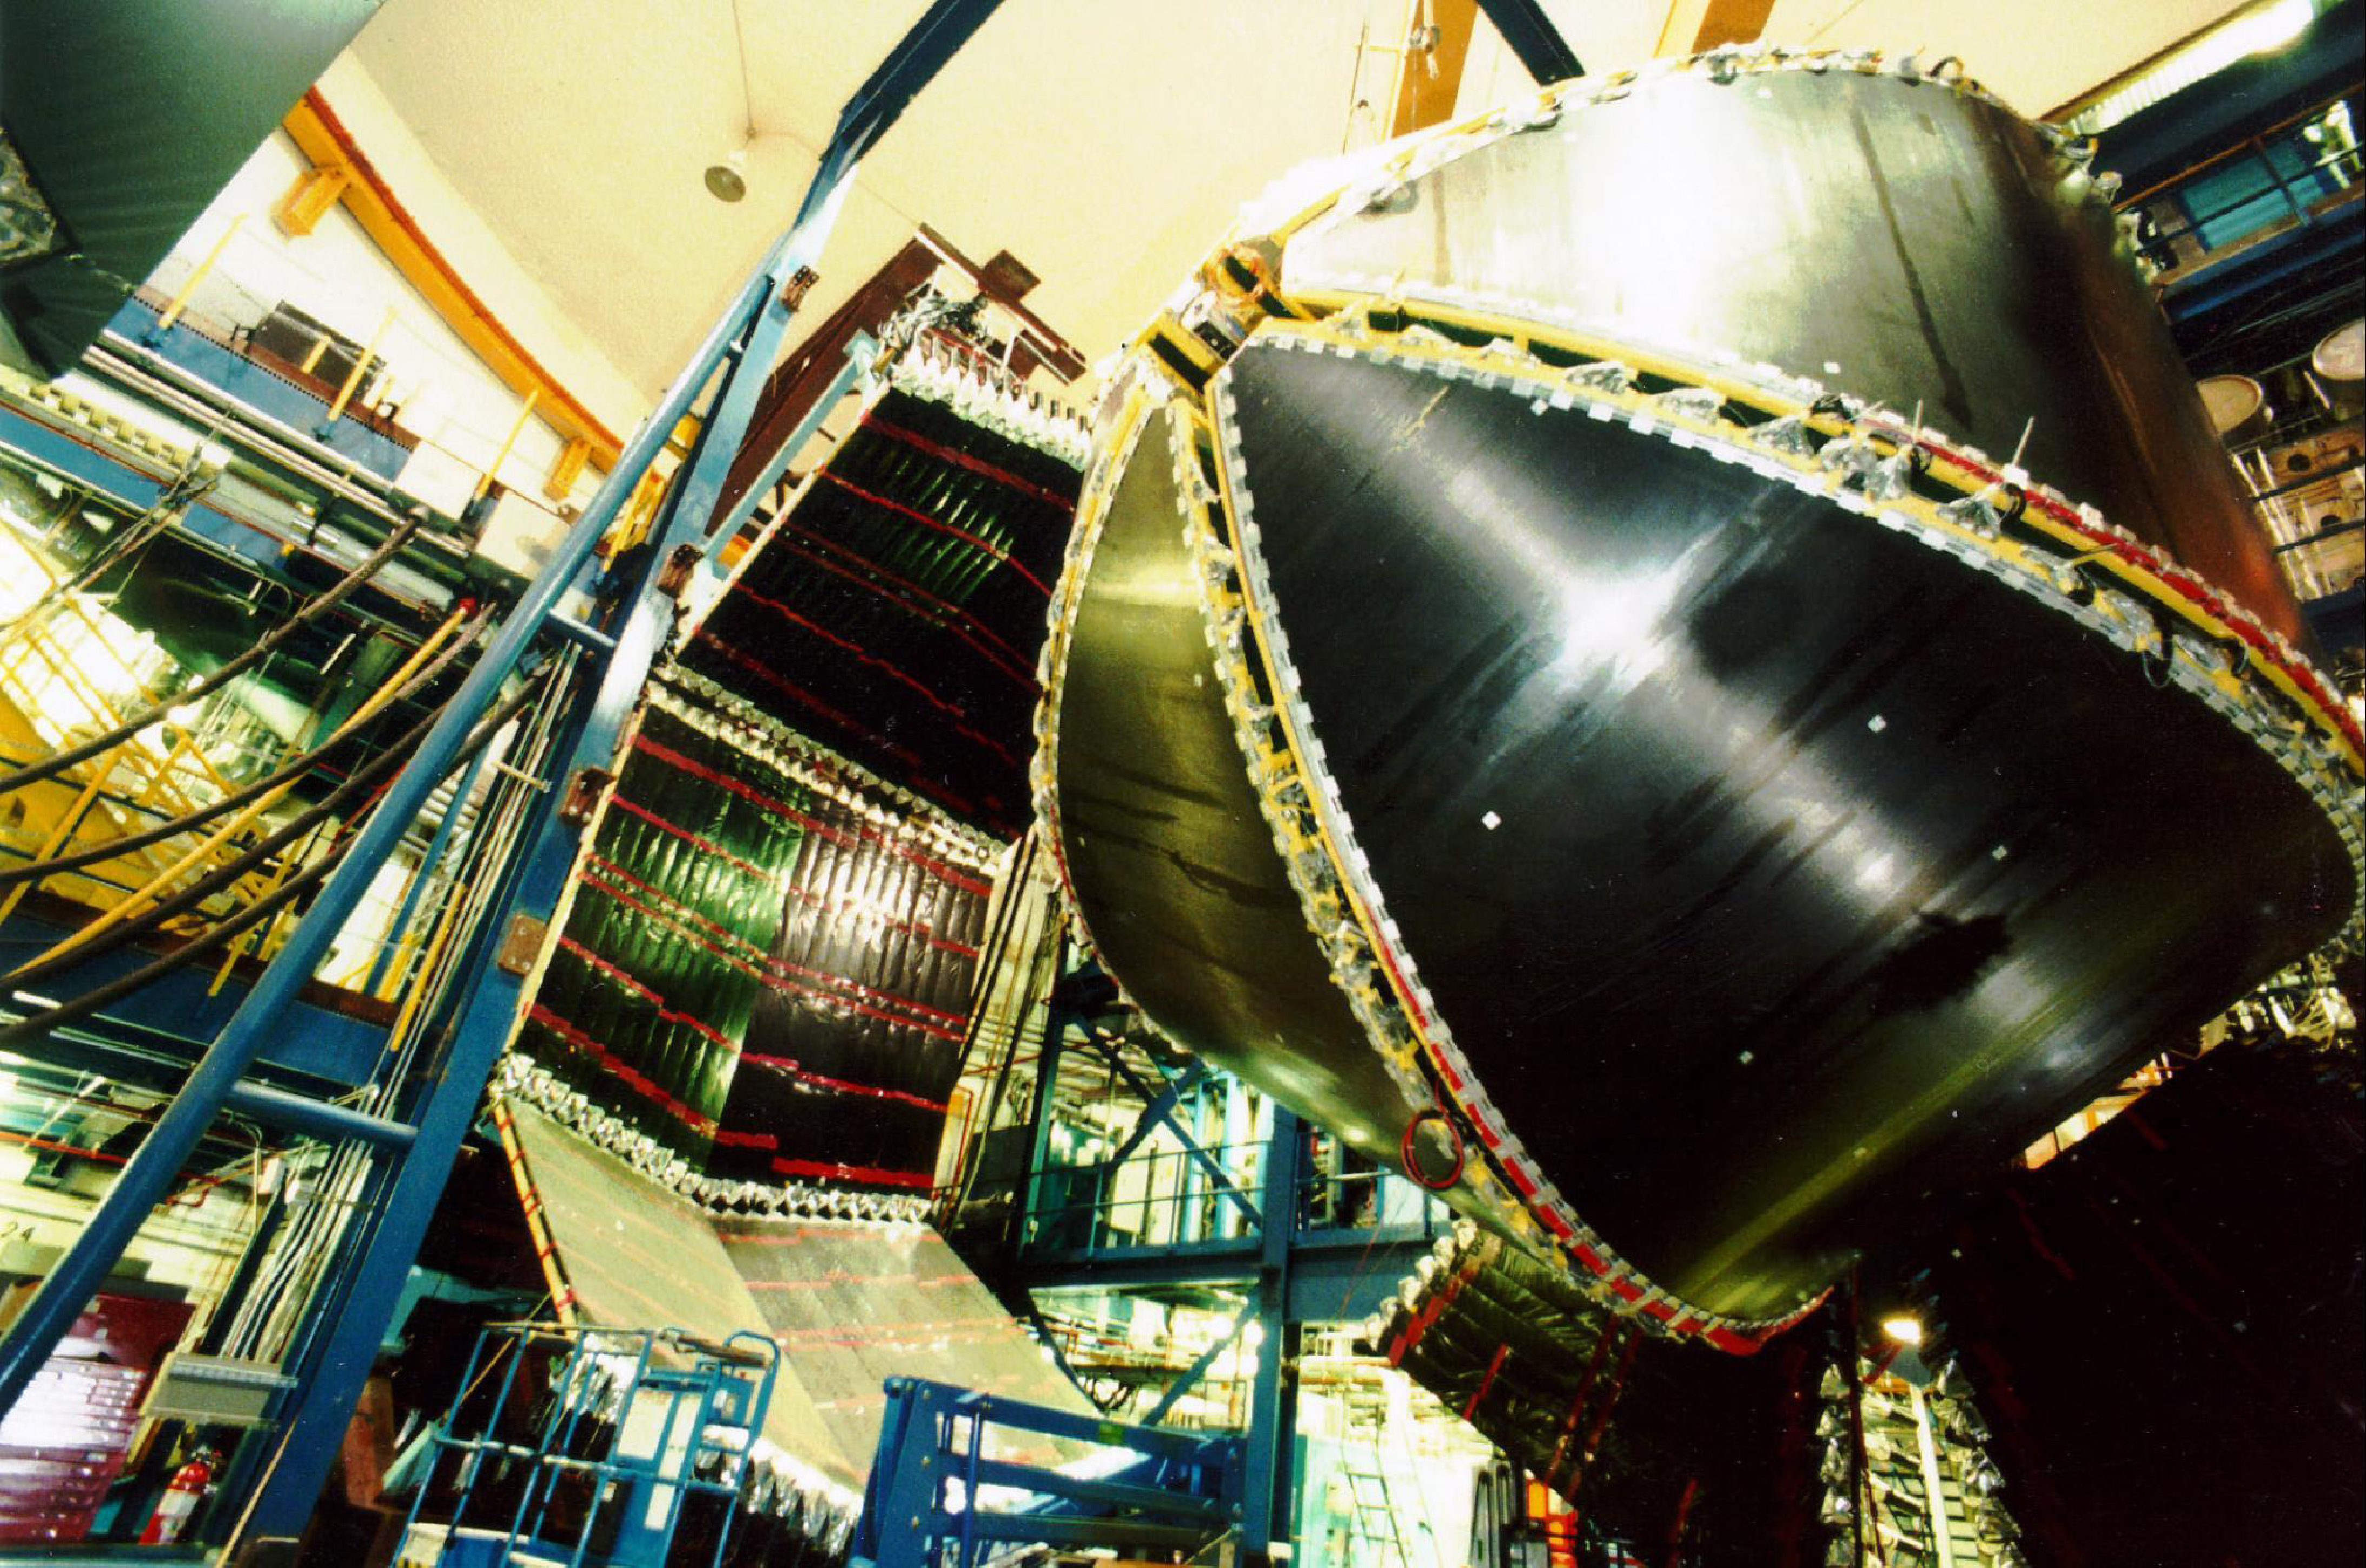
\includegraphics[width=0.8\columnwidth]{\figures/hall-b/clas_detector.pdf}
%\caption[\abbr{CLAS} Detector (photograph)]{\label{fig:clas.photo}The \abbr{CLAS} detector during a maintenance period where the time-of-flight ``shell'' (left) was pulled back from the drift-chambers (\abbr{DC}, right). The beam line enters from the lower right on the other side of the \abbr{DC}. The \abbr{TOF} paddles seen are the two center \emph{panels} shown in Fig.~\ref{fig:clas.tof.paddles} for three of the \abbr{CLAS} sectors.}
%\end{center}\end{figure}
%
%\begin{figure}\begin{center}
%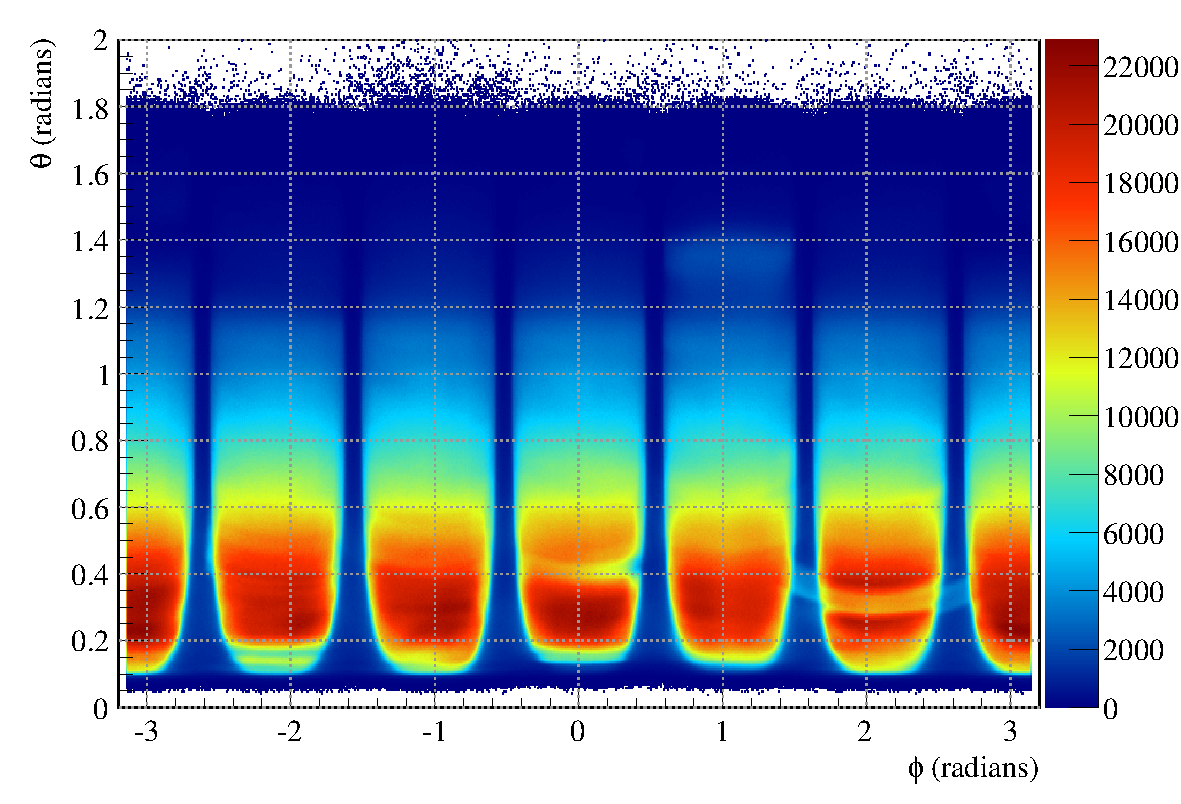
\includegraphics[width=\figwidth]{\figures/reconstruction/coverage_tof.pdf}
%\caption[Time-of-Flight Angular Coverage]{\label{fig:clas.tof.coverage}{\coloronline}Angular coverage in the lab frame of the tracks that had an associated time-of-flight hit. This can be interpreted as the total drift-chamber coverage of the \abbr{CLAS} detector.}
%\end{center}\end{figure}
